\documentclass[compress]{beamer}        % [compress] (written before {beamer} <=> navigation bar one line, all subsections in 1 line instead of 2

% Setup appearance:
\usetheme{CambridgeUS}
%	AnnArbor | Antibes | Bergen |
%	Berkeley | Berlin | Boadilla |
%	boxes | CambridgeUS | Copenhagen |
%	Darmstadt | default | Dresden |
%	Frankfurt | Goettingen |Hannover |
%	Ilmenau | JuanLesPins | Luebeck |
%	Madrid | Malmoe | Marburg |
%	Montpellier | PaloAlto | Pittsburgh |
%	Rochester | Singapore | Szeged |
%	Warsaw
%

\useoutertheme[footline=authorinstitute,subsection=false]{miniframes}
\usecolortheme{whale}

%	albatross | beaver | beetle |
%	crane | default | dolphin |
%	dove | fly | lily | orchid |
%	rose |seagull | seahorse |
%	sidebartab | structure |
%	whale | wolverine


\setbeamertemplate{footline}
{
  \hbox{%
  \begin{beamercolorbox}[wd=.25\paperwidth,ht=2.25ex,dp=1ex,center]{title in head/foot}%
    \usebeamerfont{date in head/foot}\insertshortauthor
  \end{beamercolorbox}%
  \begin{beamercolorbox}[wd=.5\paperwidth,ht=2.25ex,dp=1ex,center]{date in head/foot}%
    \usebeamerfont{title in head/foot}\insertshortinstitute
  \end{beamercolorbox}%
  \begin{beamercolorbox}[wd=.25\paperwidth,ht=2.25ex,dp=1ex,center]{title in head/foot}%
    \usebeamerfont{date in head/foot}
    \insertframenumber{} / \inserttotalframenumber
    %\insertframenumber{} / \insertpresentationendpage
  \end{beamercolorbox}}%
  \vskip0pt%
}

%\setbeamercolor{titlelike}{parent=structure}
%\setbeamercolor{structure}{fg=beamer@blendedblue}
%% \useinnertheme{rounded}
%\setbeamerfont{block title}{size={}}
%\usefonttheme[onlylarge]{structurebold}   % title and words in the table of contents bold
%\setbeamerfont*{frametitle}{size=\normalsize,series=\bfseries}
\setbeamertemplate{navigation symbols}{}
\setbeamercolor{frametitle}{parent=boxes, bg=white}
{ % only on titlepage


\usepackage{times}
\usepackage{amsmath,amssymb,amsthm}
\usepackage{color}
\usepackage{changepage}
\usepackage{multirow}
\usepackage[absolute,overlay]{textpos}
\usepackage{enumerate}
\usepackage{pgfpages}
\usepackage[all]{xy}
\usepackage{etex}
\usepackage{tikz}
\usetikzlibrary{shapes}
%\usepackage{handoutWithNotes}
%\pgfpagesuselayout{4 on 1}[border shrink=1mm]




\definecolor{camblue}{RGB}{26,26,89}
\definecolor{Rblue}{RGB}{0,255,255}
\definecolor{Rdarkblue}{RGB}{0,0,255}
\definecolor{Rgreen}{RGB}{0,205,0}
\definecolor{green2}{RGB}{51,204,51}
\newcommand{\tcb}{\textcolor{beamer@blendedblue}}
\newcommand{\tcbb}{\textcolor{camblue}}
\newcommand{\tcr}{\textcolor{red}}
\newcommand{\tcg}{\textcolor{gray}}
\newcommand{\tcgr}{\textcolor{green2}}
\newcommand{\tcblk}{\textcolor{black}}
\newcommand{\tcRg}{\textcolor{Rgreen}}
\newcommand{\tcRdb}{\textcolor{Rdarkblue}}
\newcommand{\tcRb}{\textcolor{Rblue}}
\newcommand{\tcw}{\textcolor{white}}
\newcommand{\m}{\phantom{-}}
\newcommand{\bp}{\tcbb{$\bullet$}\:}


\title{{\huge Statistics for Computing\\[0.1cm]MA4413}}
\author[Kevin Burke]{{\bf\\[0.5cm]{\huge Lecture 1}\\[0.2cm]\emph{Introduction / Basic Concepts, Data and Graphical Summaries}\\[1.4cm]Kevin Burke}\\[0.3cm]\tcb{kevin.burke@ul.ie}}

\institute[University of Limerick, Maths \& Stats Dept]{}
\date{}

%\TPGrid[5mm,5mm]{1}{1}

\begin{document}


\begin{frame}[t]
\titlepage
\end{frame}

%
%\section[Outline]{Outline}
%\subsection{Timetable and Plan}
%\begin{frame}{\bf \tcb{Timetable and Plan}\\[-1cm]}
%\begin{columns}
%
%\begin{column}{.5\textwidth}
%\begin{adjustwidth}{-0.3cm}{0.0cm}
%\begin{itemize}\itemsep0.6cm
%\item {\bf Week 1}
%\begin{itemize}\itemsep0.2cm
%\item \underline{Lecture 1}: Tuesday (11-12).
%\item \emph{No tutorials.}
%\item \emph{No Friday lecture.}
%\end{itemize}
%\item {\bf Week 2}
%\begin{itemize}\itemsep0.2cm
%\item \underline{Lecture 2}: Tuesday (11-12).
%\item \underline{Lecture 3}: \emph{in tutorial slots}\\{\scriptsize(Go to your assigned tutorial)}
%\begin{itemize}\itemsep0.05cm
%\item Tuesday (2-3).
%\item Wednesday (11-12).
%\item Friday (1-2).
%\end{itemize}
%\item \underline{Lecture 4}: Friday (3-4).
%\end{itemize}
%\end{itemize}
%\end{adjustwidth}
%\end{column}
%
%\begin{column}{.5\textwidth}
%\begin{adjustwidth}{-0.4cm}{0.0cm}
%\vspace{0.2cm}
%\begin{itemize}
%\item {\bf Weeks 3 - 12}
%\begin{itemize}\itemsep0.1cm
%\item Lectures and tutorials run as per timetable.\\[0.3cm]
%\end{itemize}
%\end{itemize}
%\begin{scriptsize}
%\begin{center}
%\begin{tabular}{|c|c|c|c|}
%\hline &&& \\[-0.2cm]
%Time  & Tuesday  & Wednesday & Friday \\[0.1cm]
%\hline &&& \\[-0.2cm]
%11am & {\bf Lecture}  & Tutorial  & \\
%12pm          & DG016    & C1058     & \\[0.1cm]
%\hline &&& \\[-0.2cm]
%12pm &&&\\
%1pm  &&&\\[0.1cm]
%\hline &&& \\[-0.2cm]
%1pm       &          &           & Tutorial \\
%2pm       &          &           & SG18     \\[0.1cm]
%\hline &&& \\[-0.2cm]
%2pm       & Tutorial &           & \\
%3pm       & C1061    &           & \\[0.1cm]
%\hline &&& \\[-0.2cm]
%3pm       &          &           & {\bf Lecture} \\
%4pm       &          &           & FG042 \\[0.1cm]
%\hline
%\end{tabular}
%\end{center}
%\end{scriptsize}
%\end{adjustwidth}
%\end{column}
%
%\end{columns}
%
%\end{frame}

%
%\subsection{Plan}
%\begin{frame}{\bf \tcb{Plan}}
%
%\begin{itemize}\itemsep0.5cm
%\item {\bf Week 1}
%\begin{itemize}\itemsep0.1cm
%\item Lecture 1: Tuesday (11-12).
%\item \emph{No tutorials.}
%\item \emph{No Friday lecture.}
%\end{itemize}
%\item {\bf Week 2}
%\begin{itemize}\itemsep0.1cm
%\item Lecture 2: Tuesday (11-12).
%\item Lecture 3 \emph{will be held in tutorial slots}:\\{\scriptsize(Go to your assigned tutorial)}
%\begin{itemize}
%\item Tuesday (2-3).
%\item Wednesday (11-12).
%\item Friday (1-2).
%\end{itemize}
%\item Lecture 4: Friday (3-4).
%\end{itemize}
%\item {\bf Weeks 3 - 12}
%\begin{itemize}\itemsep0.1cm
%\item Lectures and tutorials run as normal.
%\end{itemize}
%\end{itemize}
%
%\end{frame}


%
\section[Outline]{Outline}
\subsection{Timetable}
\begin{frame}{\bf \tcb{Timetable}\\[-1cm]}

\begin{scriptsize}
\begin{center}
\begin{tabular}{|r@{\,\,}l|c|c|c|}
\hline &&&& \\[-0.2cm]
\multicolumn{2}{|c|}{Time}  & Monday  & Thursday & Friday \\[0.1cm]
\hline &&&& \\[-0.2cm]
9 --& 10 &  {\bf Lec} CSG001 & & \\[0.1cm]
\hline &&&& \\[-0.2cm]
10 --& 11 &&& \\[0.1cm]
\hline &&&& \\[-0.2cm]
11 --& 12 &&& \\[0.1cm]
\hline &&&& \\[-0.2cm]
12 --& 1 &&& \\[0.1cm]
\hline &&&& \\[-0.2cm]
1 --& 2 &&& \\[0.1cm]
\hline &&&& \\[-0.2cm]
2 --& 3 &&& \\[0.1cm]
\hline &&&& \\[-0.2cm]
3 --& 4 & {\it Tut}: KBG11 &       & {\bf Lec}: FB028 \\[0.1cm]
\hline &&&& \\[-0.2cm]
4 --& 5 &&& \\[0.1cm]
\hline &&&& \\[-0.2cm]
5 --& 6  &         &  {\it Tut}: A1053       & \\[0.1cm]
\hline
\end{tabular}
\end{center}
\end{scriptsize}
%
%\begin{itemize}\itemsep0.6cm
%\item Tutorials start in Week 3 - \emph{Go to your assigned tutorial!}
%\end{itemize}


\end{frame}




%
%\subsection{Tutorials}
%\begin{frame}{\bf \tcb{Tutorials}}
%
%As mentioned, tutorials begin in their \emph{usual format} in Week 3.\\{\footnotesize(But don't forget to go to your tutorial in Week 2 which will be used as a lecture!)} \\[0.4cm]
%
%The usual format?
%\begin{itemize}\itemsep0.3cm
%\item Tutorial sheets will be available on the previous week.\\ {\footnotesize(e.g., Week 3 tutorial will be available in Week 2)}
%\item Based on content covered in lectures from the previous week.\\
%{\footnotesize(e.g., Week 3 tutorial will be based on Week 2 lectures)}
%\item {\bf Attempt some questions before coming to your tutorial.}
%\item Attendance will be taken.
%\item Solutions will be available at the end of the week to \emph{all students} whether they have attended or not.\\
%    {\footnotesize(e.g., Week 3 solutions will be available on Friday of Week 3)}
%\end{itemize}
%
%\end{frame}


\subsection{Tutorials}
\begin{frame}{\bf \tcb{Tutorials}}


\begin{itemize}\itemsep1.1cm
\item Tutorials begin in Week 2 (next week!)
\item Go to your assigned tutorial - ensures manageable class sizes
\item Make sure you print the tutorial sheet!
\item {\bf Try to attempt some questions before coming to your tutorial}
\item Solutions will be available to \emph{everybody} at the end of each week
\end{itemize}

\end{frame}


%
%\subsection{Tutorials: Attempting Questions}
%\begin{frame}{\bf \tcb{Tutorials: Attempting Questions}}
%There is not much point in coming to class without having made some effort at doing the questions yourself first.\\[0.5cm]
%The purpose of tutorials is to get a handle on any issues you are having with the course material.\\[0.5cm]
%\emph{Full solutions} will be available to \emph{everybody} at the end of each week; thus, your aim in tutorial classes is \emph{not} simply ``getting the solutions''.\\[0.5cm]
%You should be prepared to engage in the classes by asking questions and also answering questions (don't worry - not on the board).\\[0.5cm]
%If you are unsuccessful in your attempt at the questions, \emph{do not} feel as though you cannot come to the class - \emph{you can}! The atmosphere should be relaxed. You can still engage in the class and ask questions.
%\end{frame}
%
%
%\subsection{Tutorials: Attendance}
%\begin{frame}{\bf \tcb{Tutorials: Attendance}}
%Attend the tutorial class that you have been assigned to - this ensures that class sizes remain manageable.\\[0.5cm]
%If you wish to permanently swap to another tutorial group, email me: \tcb{ kevin.burke@ul.ie}.\\[0.5cm]
%If, \emph{occasionally}, you cannot make your usual tutorial slot (for whatever reason), just go to another slot. You do not need to tell me. Try not to let this become a frequent occurrence.\\[0.5cm]
%Attendance will be taken in tutorials. This is not worth marks towards your final exam. You are \emph{not} being forced to come to class. It's mainly for me to get to know the groups and keep an eye on the number of attendees. So no need to sign your friends in!
%\end{frame}

\subsection{Course Content: SULIS}
\begin{frame}{\bf \tcb{Course Content: SULIS}}
All content (lecture slides, tutorial sheets, solutions and any other relevant material) will be available on the SULIS website:\\[1cm]

\begin{center}
\boxed{\,\text{\tcb{http://sulis.ul.ie}}\,}\\[1cm]
\end{center}

If you have any trouble accessing the material, let me know straight away.

\end{frame}

\subsection{Assessment}
\begin{frame}{\bf \tcb{Assessment}}
\begin{columns}
\begin{column}{.7\textwidth}
There will be \emph{two} midterm exams:\\
\begin{itemize}\itemsep0.3cm
\item {\bf Friday Week 5 - October 10th.}
\item {\bf Friday Week 10 - November 14th.}
\item Likely format: 15 multiple choice questions
\phantom{Likely format:} each worth 1\%.\\[0.6cm]
\end{itemize}
\begin{enumerate}[$\Rightarrow$]
\item Midterm 1 + Midterm 2 $=$  15\% + 15\% = 30\% of the overall module.\\[0.3cm]
\item There will be a 10\% assignment during the year.
{\footnotesize (using the ``R'' programming language)}\\[0.3cm]
\item The final exam is then worth 60\%.
\end{enumerate}
\end{column}
\begin{column}{.3\textwidth}
\begin{adjustwidth}{0.3cm}{0cm}
\vspace{-1.2cm}
Grading bands:\\[0.2cm]
\begin{small}
\begin{itemize}\itemsep0.05cm
\item {\bf A1}: 90 - 100
\item {\bf A2}: 80 - 89
\item {\bf B1}: 70 - 79
\item {\bf B2}: 60 - 69
\item {\bf B3}: 55 - 59
\item {\bf C1}: 50 - 54
\item {\bf C2}: 45 - 49
\item {\bf C3}: 40 - 44
\item {\bf D1}: 35 - 39
\item {\bf D2}: 30 - 34
\item {\bf F\phantom{1}}: 0 - 29
\end{itemize}
\end{small}
\end{adjustwidth}
\end{column}
\end{columns}
\begin{textblock}{1}(11.2,2.5)
\rule{0.03cm}{6.8cm}
\end{textblock}
\end{frame}



\subsection{Maths Learning Centre}
\begin{frame}{\bf \tcb{Maths Learning Centre}}
You may or may not be aware of the Maths Learning Centre (MLC) in UL (see \tcb{http://www.mlc.ul.ie} for details).\\[1cm]
This is a drop-in centre where any student can come for one-to-one help with maths problems in room {\bf A2-018} (think of it as a free grind).\\[1cm]
This facility is open 10am-12pm and 2pm-4pm everyday during Weeks 3 - 12. It is also open in Weeks 1 and 2 on a limited basis (see website).%\\[0.7cm]
%In particular, I will be there on {\bf Wednesdays (2pm-4pm)} and {\bf Fridays (10am-12pm)} during Weeks 3 - 12. Feel free to come in if you are having difficulties.
\end{frame}



\subsection{Final Word on the Course}
\begin{frame}{\bf \tcb{Final Word on the Course}}
\begin{itemize}\itemsep1cm
\item Do not make the course more difficult for yourself.
\item Each week builds on the last. Stay on top of things - do not let them build up.
\item As soon as you have an issue, make sure you address it (at the end of a lecture, during a tutorial class, by going to the maths learning centre or by emailing me).
\end{itemize}
\end{frame}


\section{R: Statistical Programming Language}
\subsection{R: Statistical Programming Language}
\begin{frame}{\bf \tcb{R: Statistical Programming Language}}
``R'' is a widely-used \emph{freely-available} statistical programming language.\\[0.6cm]
The R code required to perform the various statistical methods covered will be provided in the lecture slides.\\[0.6cm]
Familiarity with the language will allow you (for example) to check your tutorial answers and to get a better feel for the methods.\\[0.6cm]
Statistical programmers are always highly sought after (e.g., in finance, scientific research, the pharmaceutical industry, betting companies, online companies - Google, Facebook, Amazon etc.). So a basic knowledge of R is useful at this stage.\\[0.8cm]
Note: Later in the year there will be an R based assignment (10\%).
\end{frame}

\subsection{How to Install R}
\begin{frame}{\bf \tcb{How to Install R}}
\begin{enumerate}[1.]\itemsep0.6cm
\item Go to \tcb{http://cran.r-project.org/} and click on ``Download R for Windows'' at the top of the main page.
\item On the next page click ``install R for the first time''.
\item At the top of the next page click ``Download R for Windows''. %(the latest version at the time of writing).
\item Run the downloaded executable file to install R on your computer.
\end{enumerate}
\end{frame}

\subsection{Using R - Basic Example}
\begin{frame}{\bf \tcb{Using R - Basic Example}}
Now that you have installed R, click on the R icon to open it.\\[0.3cm]
Once open, click on ``File'' in the top left corner and then ``New script''.\\[0.3cm]
Copy and paste the code below into the script that you have opened:\\
\begin{center}
\begin{tabular}{|l|}
\hline
\texttt{x = c(1,1,2,4,3,2,1,4,5,3,6,9,1,2,15)}\\
\texttt{mean(x)}\\
\texttt{sd(x)}\\
\hline
\end{tabular}
\end{center}
Within this script file in R, highlight the copied code. Press ``Ctrl + R'' to run it.\\[0.3cm]
This gives the \emph{mean} and \emph{standard deviation} (more on these later) for the vector of numbers stored in \texttt{x} - you should get 3.933333 and 3.788454 in the R console.
\end{frame}

\subsection{Using R - More Information}
\begin{frame}{\bf \tcb{Using R - More Information}}
If you wish to learn more about R, there are many options:
\begin{itemize}\itemsep0.6cm
\item Within your R script you can use the ``\texttt{?}'' command to find out more about a given function, e.g., running the code \boxed{\text{\texttt{?mean}}} will tell you about the \texttt{mean} function.
\item At the top of the R window you will see a ``help'' menu. Here you can find information about various aspects of R. In particular, under the heading ``Manuals (in PDF)'', the ``An Introduction to R'' and ``R Reference Manual'' are useful.
\item There is extensive information about R online, e.g., google ``R tutorial'' or ``R beginners guide'' etc. There are also R help forums where many solutions to common problems can be found.
\end{itemize}
\end{frame}


\section{Statistics}
\subsection{Population of Interest}
\begin{frame}{\bf \tcb{Population of Interest}}
\begin{itemize}\itemsep0.2cm
\item Statistics is the collection and analysis of data.
\item Based on our analysis we make conclusions about a {\bf population} of interest.
\item These conclusions then allow us to make \emph{informed} decisions.\\[0.8cm]
\end{itemize}
For example, let's say we are interested in the average income of a recent UL graduate (1-3 years since graduation say).\\[0.5cm]

The {\bf population} is \emph{all} previous UL students who graduated in the last 3 years.\\[0.5cm]

Can we contact every individual in the population?
\end{frame}

\subsection{Representative Sample}
\begin{frame}{\bf \tcb{Representative Sample}}
Can we contact every individual in the population? - {\bf No!} This is very rarely possible. Even if it was possible, it is unnecessary, time-consuming and expensive. We can understand the population \emph{without} seeing it in its entirety.\\[0.6cm]
Instead we work with a {\bf sample} of individuals from the population of interest; we may contact 100 recent graduates for example.\\[0.6cm]
Of course, we must be careful about how we collect our sample. It must be {\bf representative} of the population in question.\\[0.6cm]
For example, if we only asked computer science graduates about their income level, our sample would not represent the specified population - \emph{all graduates} - leading to biased results.
\end{frame}

\subsection{Random Sampling}
\begin{frame}{\bf \tcb{Random Sampling}}
We must use a {\bf random sampling} method to ensure that a representative sample is selected $\Rightarrow$ {\bf unbiased results}.\\[0.6cm]
Random sampling is any method whereby all individuals in the population have an equal chance of being selected.\\[0.6cm]
For example, let's assume that 10,000 students have graduated in the last 3 years. We can assign a number to each graduate (1-10,000) and then use a random number generator to select 100 numbers in the range 1-10,000. This produces a random sample of 100 graduates.\\[0.6cm]
In R this can be achieved via \boxed{\text{\texttt{sample(1:10000,size=100)}}}.\\[0.2cm]
Of course it is also possible using C or Java.
\end{frame}


\subsection{Parameter Vs Statistic}
\begin{frame}{\bf \tcb{Parameter Vs Statistic}}
We are interested in some feature of the population (average income of a UL graduate from our previous example).\\[0.5cm]
The true value of this feature is known as the {\bf parameter}, i.e., the value based on the \emph{whole} population.\\[0.5cm]
The parameter value is \emph{unknown} and must be \emph{estimated from the sample}.\\[0.5cm]
Our estimate of the parameter is called the {\bf statistic}, i.e., the value calculated using our sample. For example, the average income in our sample of 100 graduates.\\[0.7cm]
Memory Aid: \emph{``P'' is for population and parameter.\newline
\phantom{Memory Aid:} ``S'' is for sample and statistic.}
\end{frame}

\subsection{Parameter Vs Statistic: Symbols}
\begin{frame}{\bf \tcb{Parameter Vs Statistic: Symbols}}
It is important to know the symbols used to denote particular features of interest. In this course we deal with {\bf proportions} and {\bf means}.

\begin{itemize}\itemsep0.4cm
\item {\bf Proportion}
\begin{itemize}\itemsep0.2cm
\item \emph{Examples}: the proportion of unemployed individuals, of individuals in favour of some government policy, of viruses classed as ``high-threat'', of times a user wins in online poker etc.
\item \emph{Parameter:} The population proportion is {\boldmath$p$}.
\item \emph{Statistic:} The sample proportion is {\boldmath$\hat p$} (pronounced ``p-hat'').
\end{itemize}
\item {\bf Mean} (i.e., the arithmetic average)
\begin{itemize}\itemsep0.2cm
\item \emph{Examples:} the mean income of UL graduates, annual rainfall, lifetime of a laptop, age of users of some Android application, number bugs in some piece of software etc.
\item \emph{Parameter:} The population mean is {\boldmath$\mu$} (the Greek letter ``mu'').
\item \emph{Statistic:} The sample mean is {\boldmath$\bar x$} (pronounced ``x-bar'').
\end{itemize}
\end{itemize}

\end{frame}


\subsection{Diagrammatic Explanation}
\begin{frame}{\bf \tcb{Diagrammatic Explanation}}
\begin{displaymath}
\xymatrixcolsep{1.5cm}
\xymatrixrowsep{2cm}
    \xymatrix{
    \boxed{\text{\Huge Population}} \ar@{->}[r] \ar@/_2.2pc/[d]\ar@/_1.5pc/[d]\ar@/_0.8pc/[d]\ar@{->}[d]\ar@/^0.8pc/@{->}[d]\ar@/^1.5pc/@{->}[d]\ar@/^2.2pc/[d] &
    \begin{tikzpicture}[baseline=(char.base)]
      \node(char)[draw,shape=ellipse]{Parameter};
    \end{tikzpicture} \\
        \boxed{\text{Sample}} \ar@{->}[r] &
    \begin{tikzpicture}[baseline=(char.base)]
      \node(char)[draw,shape=ellipse]{Statistic};
    \end{tikzpicture} \ar@{.>}[u]}
\end{displaymath}

\begin{textblock}{1}(2.1,3.8)
\xymatrixrowsep{1cm}
\xymatrix{\\\ar@/^1.5pc/@{.}[u]}
\end{textblock}
\begin{textblock}{5}(2.2,3.3)
{\footnotesize\emph{The group of all individuals of interest (large in size)}}
\end{textblock}

\begin{textblock}{1}(2.7,11.4)
\xymatrixrowsep{0.7cm}
\xymatrix{&\ar@/_1pc/@{.}[ld]\\&}
\end{textblock}
\begin{textblock}{5.5}(0.5,13)
{\footnotesize\emph{A subset of individuals selected from the population (small relative to the population size)}}
\end{textblock}

\begin{textblock}{1}(1.7,10)
\xymatrixcolsep{1.5cm}
\xymatrix{&\ar@/^0.5pc/@{.}[l]}
\end{textblock}
\begin{textblock}{3.5}(0.3,7.5)
{\footnotesize\emph{Selection process must generate a representative sample}}
\end{textblock}
\begin{textblock}{3.5}(0.1,10.7)
{\footnotesize\emph{(random sampling)}}
\end{textblock}

\begin{textblock}{1}(13.4,3.8)
\xymatrixrowsep{1.3cm}
\xymatrix{\\\ar@/_1.5pc/@{.}[u]}
\end{textblock}
\begin{textblock}{4}(11.4,1.6)
{\footnotesize\emph{The true value of the feature of interest (unknown - must be estimated)}}
\end{textblock}

\begin{textblock}{1}(13,11.4)
\xymatrixrowsep{1.2cm}
\xymatrix{\\\ar@/_1.8pc/@{.}[u]}
\end{textblock}
\begin{textblock}{4.5}(9.4,13)
{\footnotesize\emph{The feature of interest calculated using the sample data}}
\end{textblock}

\begin{textblock}{1}(11.8,7)
\xymatrixcolsep{0.7cm}
\xymatrix{\\&\ar@/_0.4pc/@{.}[l]}
\end{textblock}
\begin{textblock}{3}(13.2,7.5)
{\footnotesize\emph{An unbiased statistic estimates the parameter}}
\end{textblock}
\end{frame}


\subsection{Question 1}
\begin{frame}{\bf \tcb{Question 1}}
A manager wants to estimate the proportion of faulty resistors produced (in a particular week). Individual units are selected at random times during the morning shift of each day and then tested for faults. In total 1520 resistors were tested and 18 if these were found to be faulty.\\[0.4cm]
\begin{enumerate}[a)]
\item What is the population?
\item What is the sample?
\item What is the parameter? What symbol do we use? What is its value?
\item What is the statistic? What symbol do we use? What is its value?
\item Identify any potential bias.
\end{enumerate}
\end{frame}


\subsection{Question 2}
\begin{frame}{\bf \tcb{Question 2}}
ITD wish to determine the duration of time that a UL student spends on Facebook each day. They send an email of enquiry to 500 students (by randomly selecting ID numbers) - 286 students respond. The mean time spent on Facebook in this sample was found to be 1.5 hours per day.\\[0.4cm]
\begin{enumerate}[a)]
\item What is the population?
\item What is the sample?
\item What is the parameter? What symbol do we use? What is its value?
\item What is the statistic? What symbol do we use? What is its value?
\item Identify any potential bias.
\end{enumerate}
\end{frame}

%\subsection{Question 3}
%\begin{frame}{\bf \tcb{Question 3}}
%two populations.... picture quality..\\[0.4cm]
%\begin{enumerate}[a)]
%\item What is the population?
%\item What is the sample?
%\item What is the parameter? What is its value?
%\item What is the statistic? What is its value?
%\item Identify any potential bias.
%\end{enumerate}
%\end{frame}






\section{Data}
\subsection{Data Types}
\begin{frame}{\bf \tcb{Data Types}}
There are two main types of data (the second subdivides further into two groups):\\[0.5cm]
\begin{enumerate}[1.]\itemsep0.8cm
\item {\bf Categorical}
\begin{itemize}\itemsep0.3cm
\item Labels / words which define various categories.
\end{itemize}
\item {\bf Numerical}
\begin{itemize}\itemsep0.3cm
\item {\bf Discrete}: Only a limited number of values (usually integers).
\item {\bf Continuous}: Any (decimal) value in a particular range.
\end{itemize}
\end{enumerate}

\end{frame}


\subsection{Question 3: Classify the Data Type}
\begin{frame}{\bf \tcb{Question 3: Classify the Data Type}}

\begin{itemize}\itemsep0.2cm
\item Your age in years (20, 21, 30 etc.)
\item Temperature
\item Opinion of maths (dislike, indifferent, like)
\item Processor speed (gigahertz)
\item Number of bugs in an application
\item Employment status (unemployed, employed, retired)
\item Gender (male, female)
\item Time taken to process some task
\item Distance
\item Paying attention in class (yes, no)
\item File size (gigabytes)
\end{itemize}

\end{frame}


\subsection{Categorical $\Rightarrow$ Proportions. Numerical $\Rightarrow$ Means.}
\begin{frame}{\bf \tcb{Categorical $\Rightarrow$ Proportions. Numerical $\Rightarrow$ Means.}}
Recall: the main features we deal with are {\bf proportions} and {\bf means}.\\[0.2cm]
\begin{itemize}\itemsep0.5cm
\item Categorical data: calculate the \emph{proportion} of each category. For example, consider the variable ``paying attention in class'' with two categories - ``yes'' and ``no''. We calculate the proportion of individuals paying attention and the proportion not paying attention.
\item Numerical data: calculate the \emph{mean}. For example, consider the variable ``income of a UL graduate''. We calculate the mean income.\\[0.6cm]
\end{itemize}

Note: we can also split a numerical variable by a categorical variable and \emph{compare} the means in each group, e.g., mean income for UL graduates who got a 1.1 degree versus those who got a 2.1.
\end{frame}


\subsection{Visualising Data}
\begin{frame}{\bf \tcb{Visualising Data}}

We would like to ``see'' the data. This is more helpful than attempting to eyeball the individual values - especially if we have collected a large sample.\\[0.4cm]

In particular we would like to discover the {\bf distribution of data} which describes how various categories or values are \emph{distributed}, i.e., how likely they are to occur.\\[0.6cm]

The type of data determines the type of graph:\\[0.2cm]
\begin{itemize}\itemsep0.3cm
\item Categorical data: {\bf Bar chart}
\item Numerical data: {\bf Histogram}
\end{itemize}

\end{frame}


\section{Categorical Data}
\subsection{Visualising Categorical Data}
\begin{frame}{\bf \tcb{Visualising Categorical Data}}
We first count the number of entries in each category - the frequencies - and construct a {\bf frequency table}.\\[0.4cm]
A {\bf bar chart} is simply a graph with the frequencies (or relative frequencies) on the y-axis and the category labels on the x-axis.\\[0.6cm]
Consider the following example:\\[0.2cm]
In 2011 a market researcher carried out an online survey with the intention of discovering the market share of various mobile devices. Participants were asked tick a box indicating the mobile device that they use: ``Android'', ``Apple'', ``BlackBerry'', ``Windows'' or ``Other''. In total 500 individuals were surveyed and a frequency table was constructed (see next slide).

\end{frame}




\subsection{Categorical Data: Frequency Table}
\begin{frame}{\bf \tcb{Categorical Data: Frequency Table}\\[-1cm]}
\begin{center}
Market Share 2011: Ordered highest to lowest frequency\\[0.1cm]
\begin{tabular}{|c|r|r|}
\hline
&&\\[-0.4cm]
Category   & Frequency & Relative Frequency \\
&&\\[-0.5cm]
\hline
&&\\[-0.4cm]
Android    &   174     & $\tfrac{174}{500} = 0.348$ \\[0.2cm]
Other      &   138     & $\tfrac{138}{500} = 0.276$ \\[0.2cm]
Apple      &   107     & $\tfrac{107}{500} = 0.214$ \\[0.2cm]
BlackBerry &    74     & $\tfrac{74}{500} = 0.148$ \\[0.2cm]
Windows    &     7     & $\tfrac{7}{500} = 0.014$ \\[0.2cm]
\hline
&&\\[-0.4cm]
\multicolumn{1}{|r|}{Total:} & $n = 500$ & $\tfrac{500}{500} = 1.000$ \\[0.1cm]
\hline
\end{tabular}
\end{center}
\begin{itemize}\itemsep0.2cm
\item The symbol for the total sample size is {\boldmath$n$} - we will use this throughout the course.
\item The relative frequencies (or proportions) add to 1.00. Also, these serve as estimates of the true \emph{population proportions}.
\end{itemize}

\end{frame}


\subsection{Categorical Data: Bar Chart (Frequency)}
\begin{frame}{\bf \tcb{Categorical Data: Bar Chart (Frequency)}\\[-1.1cm]}
\begin{center}
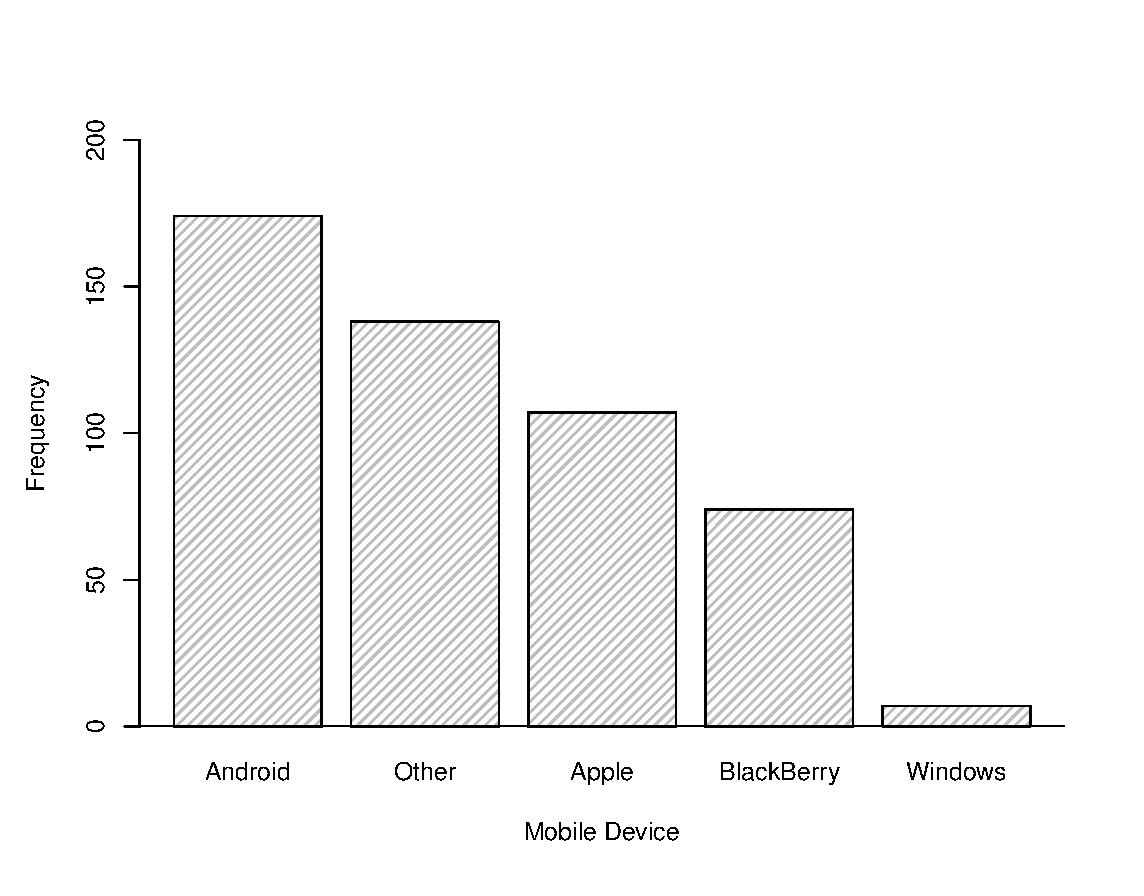
\includegraphics[width=0.8\textwidth, trim = 0.0cm 0.5cm 0.3cm 1cm, clip]{MobileDevice}
\end{center}
\begin{itemize}\itemsep0.2cm
\item Note that there are {\bf gaps} between the various categories.
\end{itemize}
\end{frame}

\subsection{Categorical Data: Bar Chart (Relative Frequency)}
\begin{frame}{\bf \tcb{Categorical Data: Bar Chart (Relative Frequency)}\\[-1.1cm]}
\begin{center}
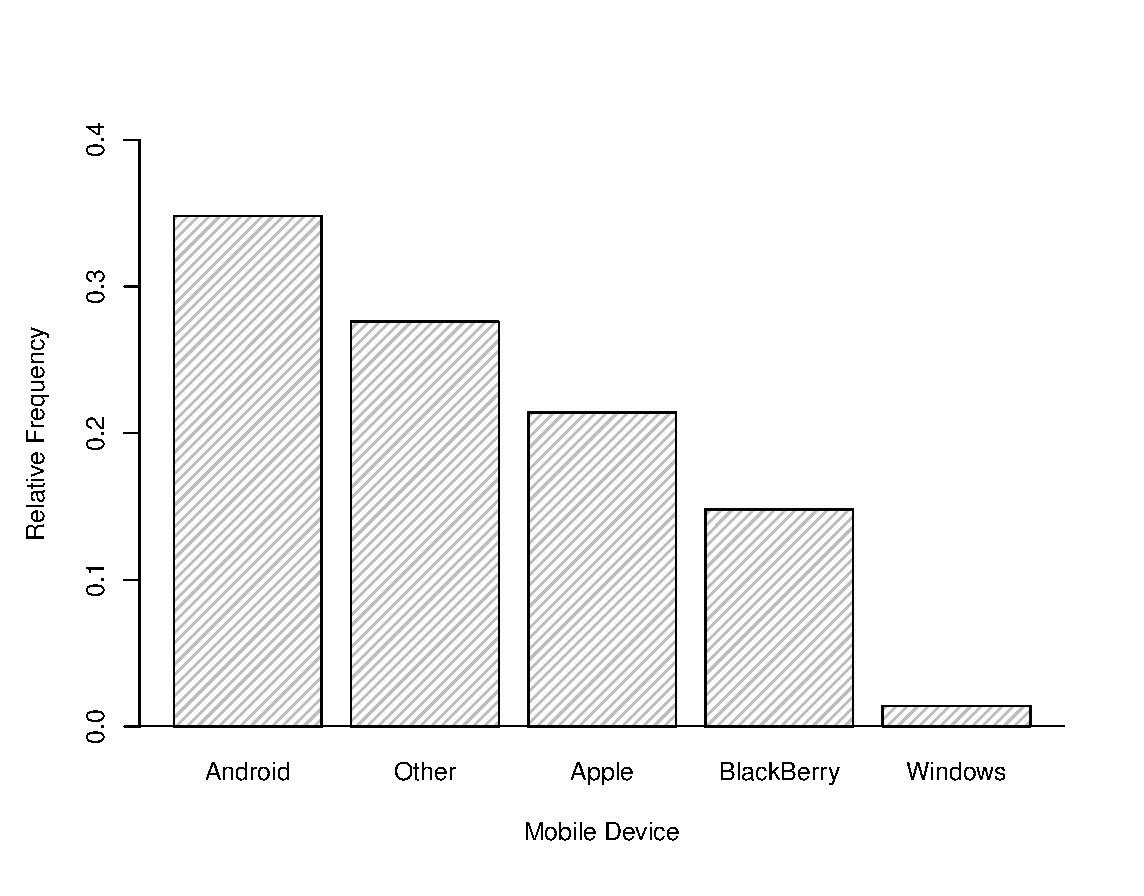
\includegraphics[width=0.8\textwidth, trim = 0.0cm 0.5cm 0.3cm 1cm, clip]{MobileDevice-Rel}
\end{center}
\begin{itemize}\itemsep0.2cm
\item Same picture but using relative frequency (see y-axis).
\end{itemize}
\end{frame}


\subsection{R Code: Bar Chart}
\begin{frame}{\bf \tcb{R Code: Bar Chart}\\[-1.1cm]}
The R code used to draw a bar chart is:\\[0.1cm]
\begin{tabular}{|l|}
\hline
\texttt{freq = c(174,138,107,74,7)}\\
\texttt{mobile = c("Android","Other","Apple","BlackBerry",}\\
\hspace{2.6cm}\texttt{"Windows")}\\
\texttt{barplot(freq, names=mobile)}\\
\hline
\multicolumn{1}{c}{}\\[-0.1cm]
\end{tabular}
You should \emph{always} label the axes:\\[0.1cm]
\begin{tabular}{|l|}
\hline
\texttt{barplot(freq, names=mobile, xlab="Mobile Device",}\\
\hspace{1.9cm}\texttt{ylab="Frequency")}\\
\hline
\multicolumn{1}{c}{}\\[-0.1cm]
\end{tabular}
Some aesthetic improvements:\\[0.1cm]
\begin{tabular}{|l|}
\hline
\texttt{barplot(freq, names=mobile, xlab="Mobile Device",}\\
\hspace{1.9cm}\texttt{ylab="Frequency",density=20)}\\
\texttt{abline(h=0)}\\
\hline
\multicolumn{1}{c}{}\\[-0.1cm]
\end{tabular}
Run \boxed{\text{\texttt{?barplot}}} for more details.
\end{frame}





\subsection{Question 4}
\begin{frame}{\bf \tcb{Question 4}\\[-0.8cm]}
The following year (2012) a survey found that 359 individuals used Android, 81 used Apple, 18 used BlackBerry, 18 used Windows and 24 used other devices.\\[0.2cm]
\begin{enumerate}[a)]\itemsep0.1cm
\item What is the value of $n$\,?
\item Construct a frequency table (ordered highest to lowest frequency) and include a column with relative frequencies.
\item Estimate the proportion of individuals who use either Android or Apple devices.
\item Estimate the proportion of individuals who use other devices. What symbol would we use for this proportion?
\item What is the \emph{true} proportion of individuals who use other devices? What symbol would we use for this proportion?
\item Draw the bar chart.
\item Comment on how the market has changed since 2011.
\end{enumerate}
\end{frame}




\section{Numerical Data}
\subsection{Visualising Numerical Data}
\begin{frame}{\bf \tcb{Visualising Numerical Data}}
We first group the values into \emph{classes} (effectively converting the data into categorical data) which allows us to construct a {\bf frequency table}.\\[0.4cm]
A {\bf histogram} is simply a graph with the frequencies (or relative frequencies) on the y-axis and the class \emph{breakpoints} on the x-axis.\\[0.6cm]
Let the following set of numerical data represent the ages of $n=30$ customers of a particular service:
\begin{center}
\begin{tabular}{|cccccccccc|}
\hline
&&&&&&&&&\\[-0.4cm]
43 & 42 & 62 & 29 & 28 & 29 & 44 & 44 & 56 & 21\\
32 & 29 & 33 & 61 & 43 & 27 & 53 & 32 & 35 & 39\\
47 & 51 & 50 & 33 & 38 & 34 & 42 & 37 & 21 & 35\\
\hline
\end{tabular}
\end{center}
We will group the above into the following classes: \\[-0.4cm]
$$19 - 27.9,\,\, 28 - 36.9,\,\, 37 - 45.9,\,\, 46 - 54.9 \text{ and } 55 - 63.9.$$\\
We then simply count the number of values contained in each class.

\end{frame}


\subsection{Numerical Data: Frequency Table}
\begin{frame}{\bf \tcb{Numerical Data: Frequency Table}}

\begin{center}
\begin{tabular}{|c|r|r|}
\hline
&&\\[-0.4cm]
Class      & Frequency & Relative Frequency \\
&&\\[-0.5cm]
\hline
&&\\[-0.4cm]
19 - 27.9  &    3     & $\tfrac{3}{30} = 0.100$ \\[0.2cm]
28 - 36.9  &   11     & $\tfrac{11}{30} = 0.367$ \\[0.2cm]
37 - 45.9  &    9     & $\tfrac{9}{30} = 0.300$ \\[0.2cm]
46 - 54.9  &    4     & $\tfrac{4}{30} = 0.133$ \\[0.2cm]
55 - 63.9  &    3     & $\tfrac{3}{30} = 0.100$ \\[0.2cm]
\hline
&&\\[-0.4cm]
\multicolumn{1}{|r|}{Total:} & $n = 30$ & $\tfrac{30}{30} = 1.000$ \\[0.1cm]
\hline
\end{tabular}
\end{center}
\begin{itemize}\itemsep0.2cm
\item Note that we {\bf do not reorder the table} from highest to lowest frequency here because the \emph{classes have a natural order} already - going from smallest to largest ages.
\end{itemize}

\end{frame}


\subsection{Numerical Data: Histogram}
\begin{frame}{\bf \tcb{Numerical Data: Histogram}\\[-1.2cm]}
\begin{center}
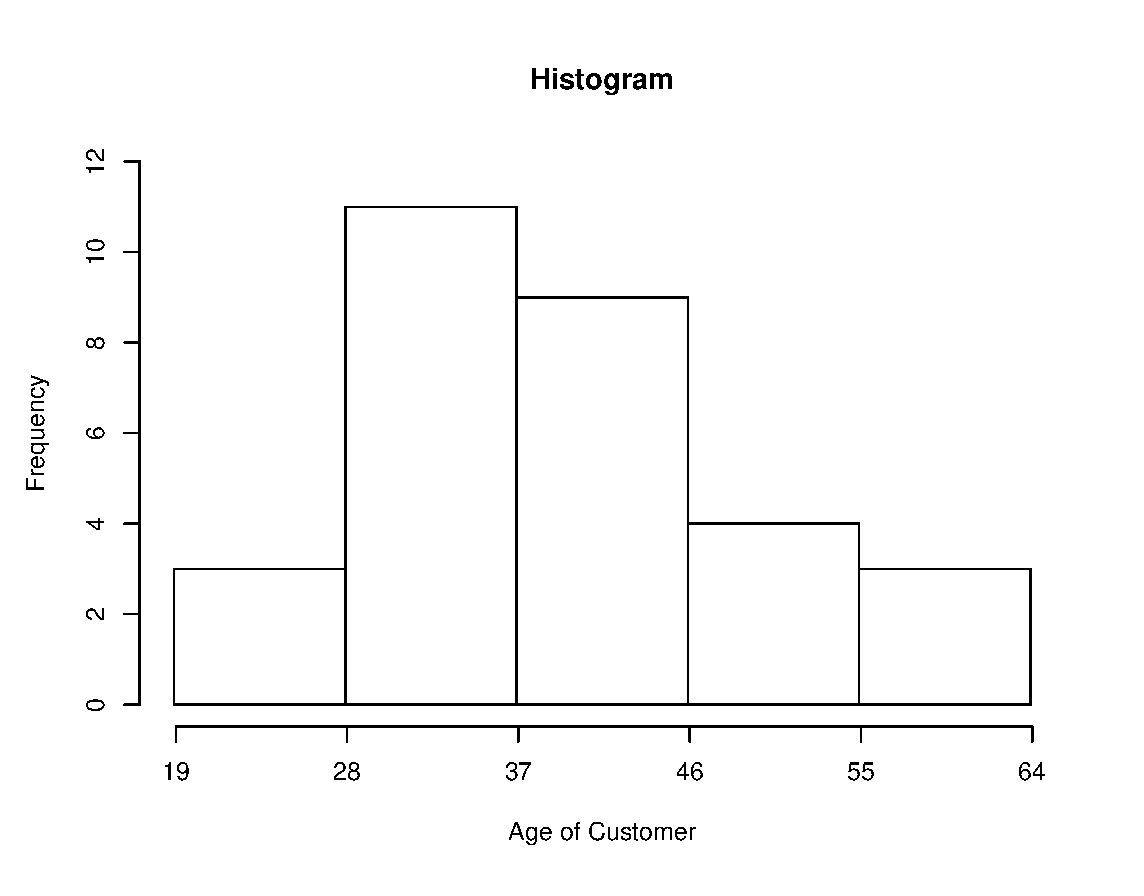
\includegraphics[width=0.8\textwidth, trim = 0.0cm 0.5cm 0.3cm 1.4cm, clip]{Ages}
\end{center}
\begin{itemize}\itemsep0.2cm
\item Note that there are {\bf no gaps} between the classes. \newline{\footnotesize(this differs from a bar chart where the groups \emph{are} separated)}
\end{itemize}
\end{frame}


\subsection{Constructing the Classes}
\begin{frame}{\bf \tcb{Constructing the Classes}\\[-0.9cm]}
\begin{enumerate}[1.]\itemsep0.6cm
\item Decide on the number of classes:
\begin{itemize}\itemsep0.4cm
\item Typically between 5 and 20 classes.
\item $\sqrt{n}$ is often a good choice.
\end{itemize}
\end{enumerate}
In our example $n=30$, so $\sqrt{30} = 5.48$ (we chose 5 classes).\\[0.7cm]
\begin{enumerate}[2.]\itemsep0.6cm
\item Calculate the class width:
\begin{itemize}\itemsep0.3cm
\item Formula: $\boxed{\text{width} = \frac{\max(x) - \min(x)}{\text{number of classes}}}$.
\item Always {\bf round up} this value (if it is not a whole number).
\end{itemize}
\end{enumerate}
In our example $\max(x) = 62$ and $\min(x) = 21$. So width is $(62-21) / 5 = 41/5 = 8.2$ $\Rightarrow$ rounded up to $9$.
\end{frame}

\subsection{Constructing the Classes}
\begin{frame}{\bf \tcb{Constructing the Classes}}
\begin{enumerate}[3.]
\item Calculate the total class range and choose the first breakpoint:
\begin{itemize}\itemsep0.3cm
\item $\text{total class range} = \text{number of classes} \times \text{class width}$.
\item We choose the first breakpoint such that the minimum and maximum data values are covered by this total class range.
\end{itemize}
\end{enumerate}

In our example the $\text{number of classes} = 5$ and $\text{width} = 9$. So the $\text{total class range} = 5 \times 9 = 45$.\\[0.2cm]
If we chose the value $0$ as the first breakpoint then the last breakpoint is $0 + 45 = 45$ giving a span of 0 - 45. Or we could choose 10 - 55. Or 15 - 60. None of these work as the span must contain the minimum and maximum data values: 21 and 62.\\[0.5cm]
Choices that work: 18 - 63,\,\, 19 - 64,\,\, 20 - 65,\,\, 21 - 66.\\[0.4cm]
In our example we chose 19 - 64.

\end{frame}

\subsection{Constructing the Classes}
\begin{frame}{\bf \tcb{Constructing the Classes}}
\begin{enumerate}[4.]
\item Construct the classes and count the number of data points contained in each.
\begin{itemize}\itemsep0.3cm
\item {\bf Every data point belongs to \emph{only one} class.}\\[0.3cm]
\end{itemize}
\end{enumerate}

In our example we have the first breakpoint $= 19$ and $\text{class width} = 9$. So the first class goes from 19 up to 19 + 9 = 28. This interval means 19 up to but \emph{not including} 28. So we say 27.9 to make this clear. The next class is then 28 up to 28 + 9 = 37 $\Rightarrow$ 36.9. \\[0.4cm]

Thus, the classes are:\\[0.3cm]

\begin{tabular}{ccccc}
\bp 19 - 27.9 & \bp 28 - 36.9 & \bp 37 - 45.9 & \bp 46 - 54.9 & \bp 55 - 63.9\\[0.2cm]
\end{tabular}

Counting the number of data points contained in these classes gives the frequency table previously shown.

\end{frame}


\subsection{R Code: Histogram}
\begin{frame}{\bf \tcb{R Code: Histogram}}
The R code used to draw the histogram is:\\[0.1cm]
\begin{tabular}{|l|}
\hline
\texttt{x = c(43, 42, 62, 29, 28, 29, 44, 44, 56, 21, 32,} \\
\hspace{1.4cm}\texttt{29, 33, 61, 43, 27, 53, 32, 35, 39, 47, 51,} \\
\hspace{1.4cm}\texttt{50, 33, 38, 34, 42, 37, 21, 35)}\\
\texttt{breakpts = c(18.9, 27.9, 36.9, 45.9, 54.9, 63.9)}\\
\texttt{hist(x, breaks=breakpts)}\\
\hline
\multicolumn{1}{c}{}\\[-0.1cm]
\end{tabular}
We can retrieve the frequencies for each class (to create the frequency table) as follows:\\[0.1cm]
\begin{tabular}{|l|}
\hline
\texttt{hist(x, breaks=breakpts)\$counts} \\
\hline
\multicolumn{1}{c}{}\\[-0.1cm]
\end{tabular}
\newline
If we do not specify breakpoints, R does it automatically:\\[0.1cm]
\begin{tabular}{|l|}
\hline
\texttt{hist(x)}\\
\hline
\multicolumn{1}{c}{}\\[-0.1cm]
\end{tabular}
\newline
Run \boxed{\text{\texttt{?hist}}} for more details.
\end{frame}

\subsection{Histogram Shape: Symmetrical}
\begin{frame}{\bf \tcb{Histogram Shape: Symmetrical}\\[-1.1cm]}
\begin{center}
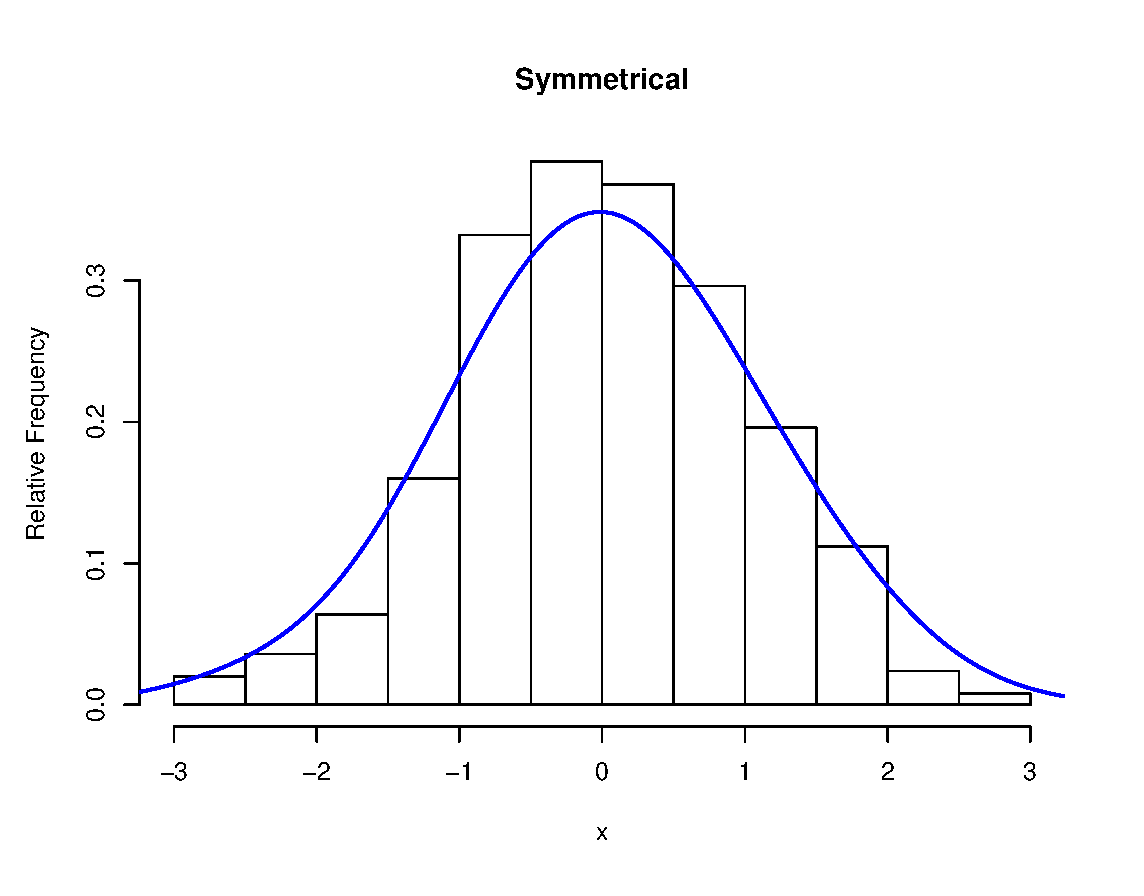
\includegraphics[width=0.8\textwidth, trim = 0.0cm 0.5cm 0.3cm 1.5cm, clip]{Symmetrical}
\end{center}
\begin{itemize}
\item Data symmetrical about the centre.
\end{itemize}
\end{frame}


\subsection{Histogram Shape: Skewed to the Right}
\begin{frame}{\bf \tcb{Histogram Shape: Skewed to the Right}\\[-1.1cm]}
\begin{center}
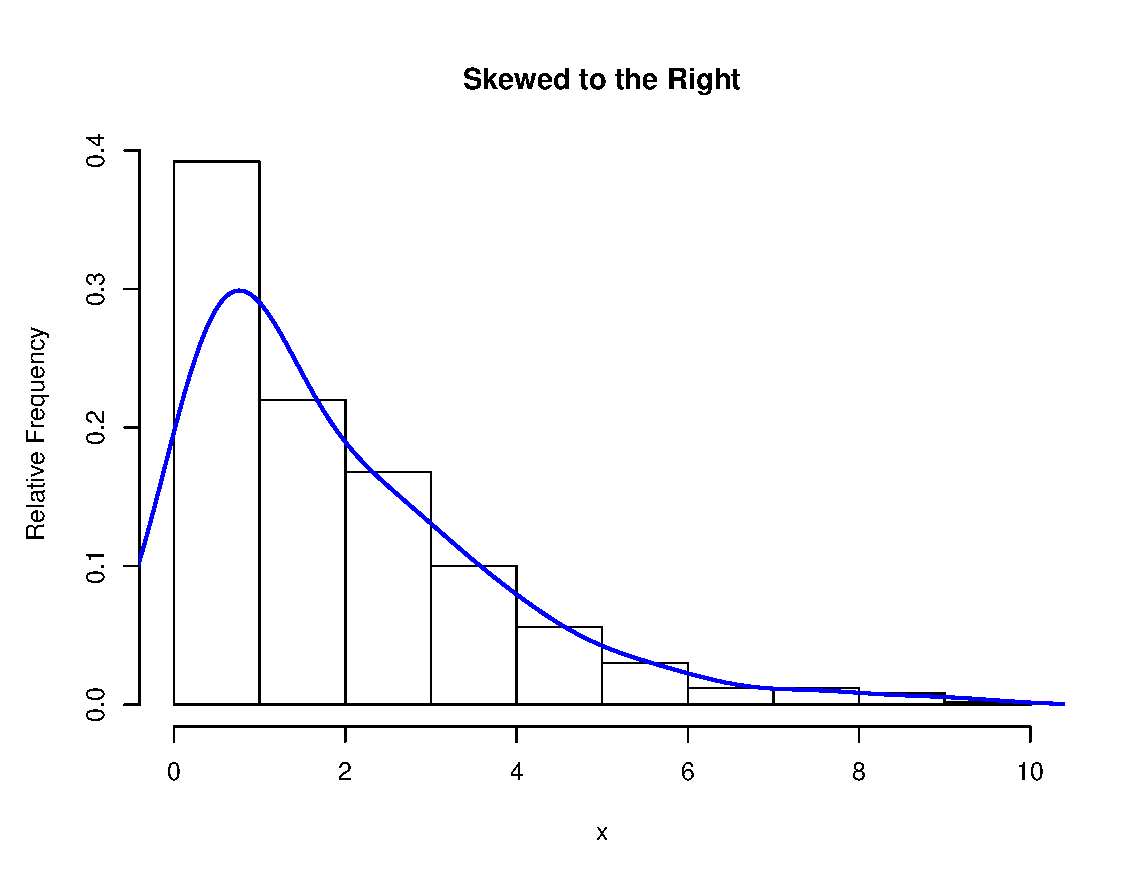
\includegraphics[width=0.8\textwidth, trim = 0.0cm 0.5cm 0.3cm 1.5cm, clip]{SkewRight}
\end{center}
\begin{textblock}{1}(10.5,9.5)
\xymatrixrowsep{0.5cm}
\xymatrix{&\ar@/_0.4pc/@{-}[ld]\\&}
\end{textblock}
\begin{textblock}{4}(12,9.1)
{\footnotesize\emph{This is the skew. \tcr{Pointing right {\boldmath$\rightarrow$}}}}
\end{textblock}
\begin{itemize}
\item A few values {\bf larger} than the main body of data.
\end{itemize}
\end{frame}


\subsection{Histogram Shape: Skewed to the Left}
\begin{frame}{\bf \tcb{Histogram Shape: Skewed to the Left}\\[-1.1cm]}
\begin{center}
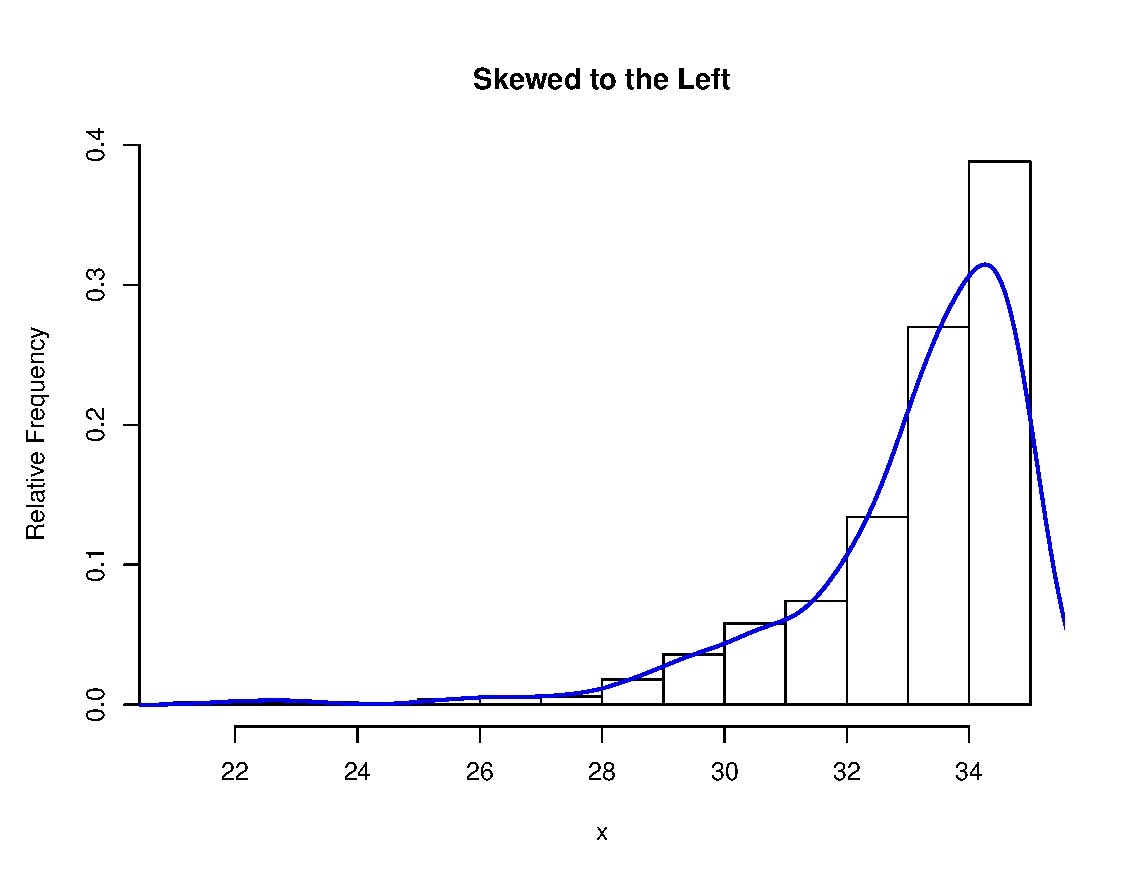
\includegraphics[width=0.8\textwidth, trim = 0.0cm 0.5cm 0.3cm 1.5cm, clip]{SkewLeft}
\end{center}
\begin{textblock}{1}(7,9.6)
\xymatrixrowsep{0.4cm}
\xymatrix{&\\&\ar@/_0.4pc/@{-}[lu]}
\end{textblock}
\begin{textblock}{4}(4.3,9)
{\footnotesize\emph{This is the skew. \tcr{Pointing left {\boldmath$\leftarrow$}}}}
\end{textblock}
\begin{itemize}
\item A few values {\bf smaller} than the main body of data.
\end{itemize}
\end{frame}


\subsection{Question 5}
\begin{frame}{\bf \tcb{Question 5}\\[-0.8cm]}
25 individuals were asked how long their laptop lasts on a full charge. The recorded times (measured in hours) are as follows:
\begin{center}
\begin{tabular}{|cccccccccc|}
\hline
&&&&&&&&&\\[-0.4cm]
2.2 & 0.4 & 4.2 & 12.9 & 1.5 & 3.0 & 5.7  & 0.7 & 1.0 & 3.3 \\
0.2 & 0.2 & 5.6 &  1.6 & 3.0 & 0.1 & 14.3 & 3.4 & 0.9 & 6.1 \\
1.4 & 1.0 & 0.7 & 5.4  & 2.3 &&&&&\\
\hline
\end{tabular}
\end{center}
\begin{enumerate}[a)]\itemsep0.1cm
\item What is the value of $n$\,? What is the value of $\bar x$?
\item Construct a frequency table with 5 classes and let zero be the first breakpoint.
    {\footnotesize(Note: the fact that the number of classes and first breakpoint are given simplifies the question)}
\item Include a column with relative frequencies.
\item Estimate the proportion of laptops that last more than 6 hours.
\item This estimated proportion is called a statistic - what is the true proportion called? What is its value?
\item Comment on the shape of the histogram.
\end{enumerate}
\end{frame}









\end{document} 